\label{chapter-scenario-template}
\textbf{Created by:} Perawit Charoenwut \\
\textbf{Modified by:}

\subsection*{Scenario Objective}
This scenario illustrates how to represent a complete company structure with manufacturing and business divisions using the IOF core ontology. It focuses on:
\begin{itemize}
    \item Showing how business and manufacturing units coexist within one company
    \item Distinguishing between business and manufacturing activities
    \item Capturing different organizational roles and functions
\end{itemize}

\subsection*{General Pattern Description}
A company can contain both business organizations and manufacturers as part of its structure.
An Organization can simultaneously be:
\begin{enumerate}
    \item A BusinessOrganization that has a BusinessFunction, which is realized through a SellingBusinessProcess that sells the MaterialProduct
    \item A Manufacturer that has a ManufacturerRole, which is realized through a ProductProductionProcess and  has the MaterialProduct as its output.
\end{enumerate}

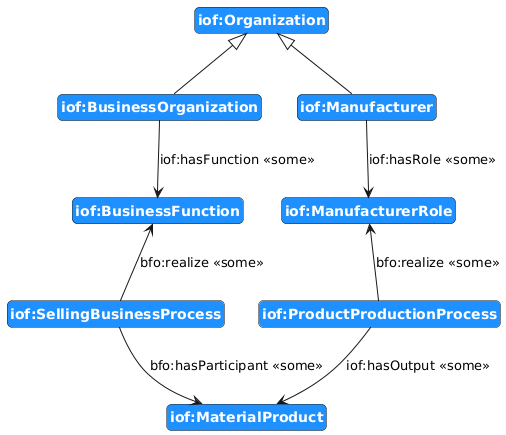
\includegraphics[scale=0.42]{scenarios/different-type-organizations/image/different-type-organizations-schema}

\subsection*{Use Case: }

This use case demonstrates how a company like GE operates as both a manufacturer and a business organization using the same material products.

\subsubsection*{Use-Case Pattern Description}

Consider GE's jet engine division, which demonstrates both manufacturing and business aspects:

\begin{itemize}
    \item As a Manufacturer: 
    \begin{itemize}
        \item Bears a ManufacturerRole
        \item Realizes this role through ProductProductionProcess
        \item Produces jet engines as MaterialProduct
    \end{itemize}
    \item As a BusinessOrganization: 
    \begin{itemize}
        \item Has BusinessFunction
        \item Realizes this through SellingBusinessProcess
        \item Sells jet engines as MaterialProduct
    \end{itemize}
\end{itemize}

\subsubsection*{Use-Case Example Data}
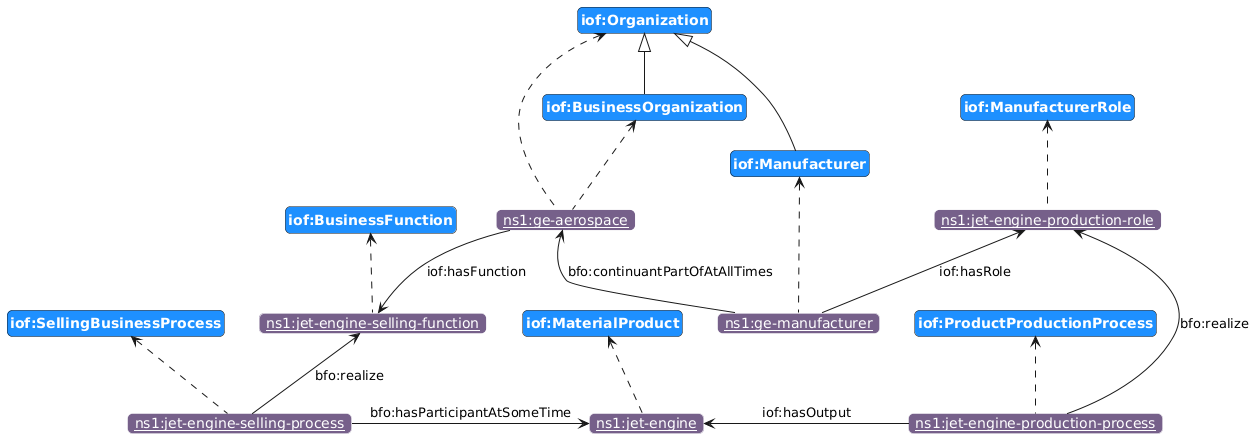
\includegraphics[scale=0.4]{scenarios/different-type-organizations/image/different-type-organizations}

\begin{table}[h]
% \caption{}
\label{tab:organization-structure}
\resizebox{\columnwidth}{!}{%
\begin{tabular}{|l|l|}
\hline
Entity & Function/Role \\ \hline
GE Aerospace & Manufactures and sells product \\
Jet engine & Product \\
Manufacturing & Manufactures product \\
Sales & Sells product \\
\hline
\end{tabular}%
}
\end{table}


\subsubsection*{Data Mapping}


\subsubsection*{Data Validation}
